\section{Real-time Animation of Sand-Water Interaction}
We all came across wet sand in one way or the other. Might is have been when building sandcastles as a child, or relaxing at the beach during a vacation. But modeling such a rather common phenomenon is much more difficult than one might expect.

\begin{figure}[htb]
	\centering
	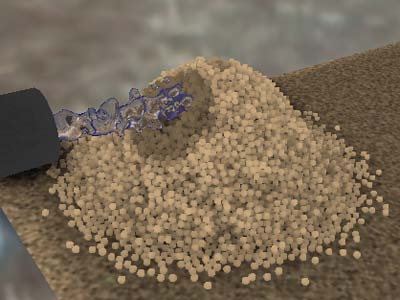
\includegraphics[width=\linewidth]{RSKN08/pileofsand.jpg}
	\caption{Calculation of sand, when water is added.}
	\label{fig:pileofsand}
\end{figure}

Although sand and beach environments are quite common in many commuter games, the physically correct simulation of sand-water interaction has only been approached recently. A very promising method was proposed by \cite{rungjiratananon2008real}. The approach is based on modeling every grain of sand as a separate particle. Each such particle as a specific "wetness" value assigned to them. This represents if we are dealing with dry, wet or "overwet" sand (see Figure \ref{fig:wetness}). Another crucial thing to take into account are the liquid bridges, which are formed between sand particles when fluids (water) are introduced.

\begin{figure}[htb]
	\centering
	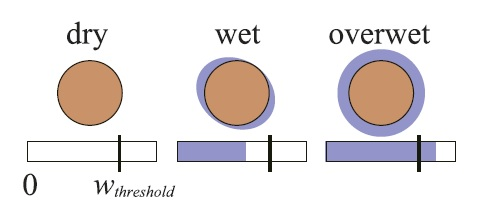
\includegraphics[width=\linewidth]{RSKN08/wetness.jpg}
	\caption{The different wetness levels of a (sand) particle.}
	\label{fig:wetness}
\end{figure}

\subsection{Two different models}
The two different models utilized here are Smoothed Particle Hydrodynamics (SPH) \cite{rungjiratananon2008real} and the Discrete Element Method (DEM) \cite{rungjiratananon2008real}.

\begin{figure}[htb]
	\centering
	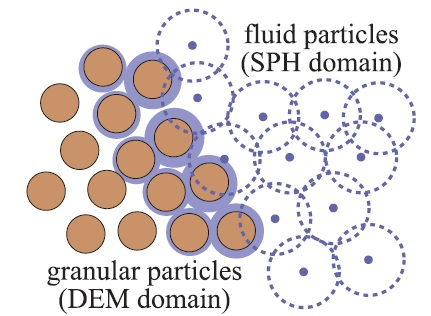
\includegraphics[width=\linewidth]{RSKN08/domains.jpg}
	\caption{Difference between DEM and SPH domain.}
	\label{fig:domains}
\end{figure}

While SPH is used to calculate forces within a particle, DEM helps calculation the attractive forces between multiple particles. If the 1st or the second model is used depends on the wetness value. exceeding a specific: If the wetness is high enough, liquid bridges are formed and therefore inter-particle forces have to be taken into account. Since those forces are quite string, gravity and moisture absorbed from the air are not considered to be part of the result and therefore not tackled in this approach.

\subsection{Performance and real-time usability}
Since every particle has to be treated completely separately resulting in a high amount of parallel computations, this is done on the GPU most efficiently. This vast number of calculations results in a "moderate" frame rate when trying to simulate more complex scenarios. The results from \cite{rungjiratananon2008real} where achieved with common Hardware from 2008, resulting in around 40 fps for 32k granular and 32k fluid particles, and drops down to 4 fps when using 33k granular and 64k fluid particles respectively.

\begin{figure}[htb]
	\centering
	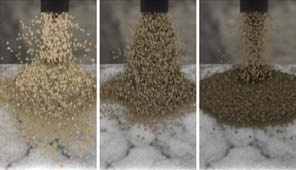
\includegraphics[width=\linewidth]{RSKN08/wetsandtypes.jpg}
	\caption{Illustration of the 3 differed wetness levels.}
	\label{fig:wetsandtypes}
\end{figure}